\scanpage{391}
\mspage{198}
lifts uniquely to
$\widehat{\widehat{\mathcal G}}^{G}$.
This should be reexamined more carefully later on.
But it seems to me that we find no new properties here of the
$\Gamma\subset\mathcal M_a$ or of
$M_a$ itself, i.e. of
$\mathbb{\Gamma}_a$ as a profinite subgroup of
$\Gamma'=\operatorname{Norm}_{\widehat{\widehat{\mathcal T}}}
(\widehat{\mathcal T})/\widehat{\mathcal T}$.

\uline{31}\quad Digression on the liftings
of \inserted{an} outer action
of\deleted{\unsure{e}}\inserted{ a} finite group $G$ on a
profinite group with loops $\pi$.
\figure{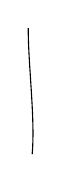
\begin{tikzpicture}[x=1cm,y=1cm,baseline=(current bounding box.south)]
\draw[line width=0.4pt] (0,0) .. controls (0.04,0.45) and (-0.05,1.12) .. (-0.05,1.60);
\end{tikzpicture}}

We assume the outer action \uline{faithful},
i.e. $G\subset\widehat{\widehat{\mathcal T}}(\pi)
=\widehat{\widehat{\mathcal T}}$,
\inserted{and that $G=G^+$.}
We assume moreover that there exists an invariant
discretification $\pi_0$, i.e. such that
$G\subset\mathcal T(\pi_0)$.

If we assume $G$ cyclic, then unless
I am mistaken it is proved that the situation is
\uline{realizable} topologically (\unsure{thus}:
\uline{\unsure{algebraically}} in a complex analytic way $\ldots$).

\scanpage{392}
In the discrete case, the meaning of the
\inserted{$\pi_0$-}conjugacy classes of lifting
$G\longrightarrow\mathcal G(\pi_0)$ is well understood;
\deleted{But}\inserted{likewise for the partial liftings}
We find a \deleted{\unsure{category} $U^{!}$} \inserted{canonical}
realization of the fundamental groupoid
\margin{if $U^{!}\ne\unsure{\varnothing|\phi}$}
associated to the
outer group $\pi_0$, by a \inserted{finite} groupoid $[U^{!}]$
on which $G$ operates in the strict sense, whose points
correspond to the $\pi_0$-conjugacy classes of
maximal partial sections $\ne1$, the group
\deleted{\illegible{1}}$\mathcal T(\pi_0)^G$
operates in an \unsure{equally} canonical way on this groupoid.
If $P\in U^{!}$ corresponds to a lifting
$G\longrightarrow\mathcal G(\pi_0)$, then
an element $\deleted{\unsure{g}}\inserted{\dot u}\in
\mathcal T(\pi_0)^G$ is in the image of
$\mathcal G(\pi_0)^G$, i.e. can be lifted to
$u\in\mathcal G(\pi_0)$ commuting with $G$, iff
$\dot u(P)=P$ [i.e. iff
\inserted{(if $\dot u$ is lifted in an \unsure{arbitrary} way to $v$)}
$v(G)$ is $\pi_0$-conjugate to $G$
i.e. iff $\exists g\in\pi_0$ such that
$v(G)=\operatorname{int}(g)(G)$
i.e. \deleted{\unsure{which}}
$u\overset{\text{definition}}{=}\operatorname{int}(g^{-1})v$ fixes $G$.
\deleted{\unsure{(Thus}} (in which case of course it centralizes,
\inserted{(by the hypothesis $\dot u\in\mathcal T^{G}$)})
Thus our brilliant assertion, is a tautology]

\scanpage{393}
\mspage{199}
and hence the lifting is unique. As
$U^{!}_{\unsure{*|\varphi}}$ is finite, hence the stabilizer
$\mathcal T(\pi_0)^G_P$ of $P$ in
$\mathcal T(\pi_0)^G$ has finite index,
and so it is this subgroup of finite index that lifts
merrily and canonically.

What can one say in the profinite context? Of course,
we have a canonical map
\diagram{\begin{tikzcd}[ampersand replacement=\&,column sep=large]
\begin{gathered}
\text{\deleted{\unsure{Set}} classes of $\pi_0$-conjugacy}\\
\text{of liftings of}\\
G\text{ into }G
\longrightarrow\mathcal G(\pi_0)\\
\text{i.e. of splittings of}\\
\text{the extension }1\longrightarrow\pi_0\longrightarrow
E\longrightarrow G\longrightarrow1
\end{gathered}
\arrow[r] \&
\begin{gathered}
\text{classes of $\pi_0$-}\\
\text{conjugacy of liftings of}\\
G\text{ into }G
\longrightarrow\widehat{\widehat{\mathcal G}}(\pi_0)\\
\text{i.e. of splittings}\\
\text{of the extension}\\
1\longrightarrow\underset{\substack{\Vert\\\pi}}{\widehat{\pi}_0}
\longrightarrow\widehat E
\longrightarrow G\longrightarrow1
\end{gathered}
\end{tikzcd}}

We should first examine

a) The question of the bijectivity of this map.

b) The question whether $\pi^G=1$ (\unsure{\uline{rigidity}|rigidity}),
for $G\ne(1)$. -- (for a given lifting,
in $E$ for simplicity)

I feel like conjecturing shamelessly
that this is so --- which would imply
for example that for every such lifting $G$, there is

\scanpage{394}

an \uline{open} subgroup \inserted{$(\unsure{\widehat{\widehat{\mathcal T}}|\widehat{\mathcal T}}^{G})_{P}$} of the group (perhaps really immense a priori!) $\widehat{\widehat{\mathcal T}}^{G}$, which lifts canonically so as to commute with \unsure{$\widetilde G$|$G$}....

We should clearly develop, at the same time as a theory of outer operations of finite groups on discrete groups with loops (which for the moment is extremely \unsure{conjectural|conjectural}) an analogous theory in the profinite case --- I \deleted{\illegible{1}}\inserted{will have} probably to come back to it later on.

\scanpage{395}
\mspage{200}

\uline{32} Return to the arithmetic aspects of plugging holes: relations between $\Gamma_{g,\nu}$ and $\Gamma_{g,\nu-1}$.

Of course, we \deleted{\unsure{see that}} have that
\[
\mathcal N_{g,\nu}\longrightarrow\mathfrak S_{\nu}
\]
is surjective \inserted{(since $\mathcal T_{g,\nu}\longrightarrow\mathfrak S_{\nu}$ is)}, hence we will have
\[
(1)\qquad 1\unsure{\longrightarrow|-}\mathcal N_{g,\nu}^{!}\unsure{\longrightarrow|-}\mathcal N_{g,\nu}\unsure{\longrightarrow|-}\mathfrak S_{\nu}\unsure{\longrightarrow|-}1
\]
and the Cartesian diagram of \unsure{subgroups} of $\widehat{\widehat{\mathcal T}}_{g,\nu}$
\[
(2)\qquad
\diagram{\begin{tikzcd}[ampersand replacement=\&]
\widehat{\mathcal T}_{g,\nu}^{+}\arrow[r,hook] \& \mathcal N_{g,\nu}\\
\widehat{\mathcal T}_{g,\nu}^{!+}\arrow[u,hook]\arrow[r,hook] \& \mathcal N_{g,\nu}^{!}\arrow[u,hook]
\end{tikzcd}}
\]
\margin{\deleted{\illegible{1}} $\mathcal N_{g,\nu}=\mathcal N_{g,\nu}^{!}\cdot\widehat{\mathcal T}_{g,\nu}^{+}$ i.e. $\mathcal N_{g,\nu}$ known from $\mathcal N_{g,\nu}^{!}$}
will give an isomorphism
\[
(3)\qquad \mathcal N_{g,\nu}^{!}/\widehat{\mathcal T}_{g,\nu}^{!+}\xrightarrow{\sim}\mathcal N_{g,\nu}/\widehat{\mathcal T}_{g,\nu}^{+}=\mathbb{\Gamma}_{g,\nu}
\]
In the case of a $(\pi,a)$, \inserted{($\pi$ an outer group with loops,} $a$ an arithmetization), we will likewise have
\[
(4)\qquad\left\{\begin{aligned}
\mathcal N_a^{!}/\widehat{\mathcal T}_a^{+}&\simeq\mathcal N_a/\widehat{\mathcal T}_a^{+}=\mathbb{\Gamma}_a.\\
\mathcal N_a&=\mathcal N_a^{!}\widehat{\mathcal T}_a^{+}
\end{aligned}\right.
\]

Let us now consider \deleted{a \unsure{subset}\inserted{\unsure{$i\in I=I(\pi)$}} , \illegible{3} $\unsure{(g,\nu)}$, \unsure{and a} $\pi_i'$ \illegible{2} $\unsure{I=I(\pi)}$, and let \illegible{1}} for $\forall i\in I$ the stabilizer \deleted{\illegible{1}} $\mathcal N_i$ of $i$ in $\mathcal N$, and the group \deleted{outer} \inserted{with loops (not outer!)} $\pi_i'$ of type $g,\nu-1$, deduced from $\pi$ by ``plugging hole $i$'',
\margin{We write $\mathcal N$ etc. instead of $\mathcal N_a$. We assume \illegible{2} $(g,\nu-1)$, i.e. \unsure{$2g-2+\nu$} \illegible{1} \unsure{$\geq1$}, i.e. $2g+\nu\geq4$}

\scanpage{396}

we then have, for a chosen discretification, \deleted{\unsure{a}} \inserted{$\alpha$} compatible with the arithmetization, an injective \unsure{homomorphism|homomorphism}
\[
(5)\qquad \pi_i'\xrightarrow{\varphi_i}\widehat{\mathcal T}_{\unsure{i|a}}^{+!}\subset\mathcal N_{\unsure{i|a}}^{!}\subset\widehat{\widehat{\mathcal T}}_i
\]

\deleted{We \unsure{cannot|can only} \illegible{2}}
\deleted{We will have}
\deleted{\unsure{which lifts the composite}}
\deleted{\textcircled{\unsure{e|c}} The image of $\pi'$}
such that the composite
\[
\diagram{\begin{tikzcd}[ampersand replacement=\&]
\pi_i'\arrow[r] \& \widehat{\widehat{\mathcal T}}_i\arrow[r] \& \widehat{\widehat{\mathcal G}}(\pi_i')\\
\&\& \pi_i'\arrow[u,hook]
\end{tikzcd}}
\]
is the canonical inclusion. This being so, we want\margin{rather: \uline{it is true that!}} the image of (5) (which may not be invariant in $\widehat{\widehat{\mathcal T}}_i$) to be \uline{invariant in \deleted{$\mathcal T$} $\mathcal N_i$}, or what amounts to the same, in $\mathcal N^{!}$ (for $\mathcal N_i=\mathcal N^{!}\cdot\widehat{\mathcal T}_i^{+}$ and $\widehat{\mathcal T}_i^{+}$ leaves this image invariant). \deleted{\illegible{1}} Returning to the universal situation, this \unsure{\uline{means}|means}
\margin{This also means that $\varphi_i$ \unsure{does not depend} on the choice of the discretification \unsure{with datum} $\alpha$...}

\textcircled{\unsure{e|c}} $\mathcal N_{g,\nu}^{!}\subset\widehat{\widehat{\mathcal T}}_{g,\nu}$ is contained in the normalizer of the $\pi_i'\hookrightarrow\widehat{\mathcal T}_{g,\nu}^{!+}$ $(0\leq i\leq\nu-1)$ \inserted{which are therefore invariant in $\mathcal N_{g,\nu}^{!}$} \deleted{\unsure{if} $(g,\nu-1)$ \unsure{is also anabelian}}.

Moreover $\widehat{\widehat{\mathcal T}}_{g,\nu}^{!}\xrightarrow{\psi_i}\widehat{\widehat{\mathcal G}}_{g,\nu-1}^{!}$ induces an \deleted{\illegible{1}} \uuline{\unsure{isomorphism|isomorphism}}
\[
(6)\qquad\mathcal N_{g,\nu}^{!}\xrightarrow{\sim}\mathcal M_{g,\nu-1}^{!}
\]
\margin{\uline{N.B.} It suffices \unsure{it seems to me} to prove it \unsure{for one $i$} to deduce it for the others \deleted{\illegible{1}}}
\margin{\uline{N.B.} \illegible{4}}

\scanpage{397}
\mspage{201}

This assertion breaks up into two: first \unsure{then|of all} that $\psi_i$ does indeed map $\mathcal N_{g,\nu}^{!}$ into $\mathcal M_{g,\nu-1}^{!}$ -- and this follows from the \unsure{arithmetico-geometric} definition of these groups -- this implies on the other hand, since $\psi_i$ also induces an \inserted{\unsure{isomorphism}} \deleted{\illegible{1}}
\[
\widehat{\mathcal T}_{g,\nu}^{+}
\xrightarrow{\sim}
\widehat{\mathcal G}_{g,\nu-1}^{+},
\]
that it induces a homomorphism
\[
(7)\qquad
\begin{array}{ccc}
\mathbb{\Gamma}_{g,\nu}
&\xrightarrow{\substack{\inserted{\lambda_i}\\\deleted{\unsure{\psi_i}}}}&
\mathbb{\Gamma}_{g,\nu-1}\\
\wr\vert&&\wr\vert\\
\mathcal N_{g,\nu}/\widehat{\mathcal T}_{g,\nu}^{+}
&&\mathcal M_{g,\nu-1}/\unsure{\widehat{\mathcal G}}
\end{array}
\]
\deleted{and by \unsure{arithmetic} means}
and the injectivity (resp. \deleted{b}\unsure{surjectivity}) of (6) is equivalent to that of (7). Moreover (7) fits, by construction, into a commutative diagram

\begin{samepage}
(8)\quad\diagram{\begin{tikzcd}[ampersand replacement=\&,column sep=large,row sep=large]
\& \mathbb{\Gamma}_{\mathbb Q}
  \arrow[dl,"\Theta_{g,\nu}"']
  \arrow[dr,"\Theta_{g,\nu-1}"] \& \\
\mathbb{\Gamma}_{g,\nu} \arrow[rr]
\&\&\mathbb{\Gamma}_{g,\nu-1}
\end{tikzcd}}
\end{samepage}

with $\Theta_{g,\nu}$ and $\Theta_{g,\nu-1}$ surjective, so it is indeed quite obvious that (6) is \uline{surjective}. Bijectivity \unsure{\uline{means}|means} that $\Theta_{g,\nu}$ and $\Theta_{g,\nu-1}$ have the same kernel (whereas a priori it could be that $\Theta_{g,\nu}$ has a smaller kernel i.e. corresponds to a representation of $\mathbb{\Gamma}_{\mathbb Q}$ ``less unfaithful'' than $\Theta_{g,\nu-1}$. Moreover,

\scanpage{398}

it is obvious \deleted{that} (\unsure{even}, a priori, without using the definition \inserted{elsewhere} \unsure{explicit|made explicit} of the $\mathcal N_{g,\nu}$) that the homomorphism $\deleted{\unsure{\psi_i}}\inserted{\unsure{\lambda_i}}$ \inserted{\unsure{(7)}} does not depend on the choice of $0\leq i\leq\nu-1$ -- for example since we pass from one to the other by applying operations of $\widehat{\mathcal T}^{+}$ (since $\widehat{\mathcal T}^{+}$ operates \unsure{transitively} on $I$) and $\widehat{\mathcal T}^{+}$ operates \unsure{trivially|trivially} on $\mathbb{\Gamma}_{g,\nu}$ ...

We can say that (6) describes $\mathcal M_{g,\nu-1}^{!}$ (hence $\mathcal N_{g,\nu-1}^{!}$) in terms of $\mathcal N_{g,\nu}$ -- but the reverse is less clear, for lack of knowing whether
\[
\unsure{\widehat{\widehat{\mathcal T}}_{g,\nu}^{!}}
\xrightarrow{\psi_i}
\widehat{\widehat{\mathcal G}}_{g,\nu-1}
\]
is injective; if we knew this, we could describe $\mathcal N_{g,\nu}^{!}$ as the inverse image of $\mathcal M_{g,\nu-1}^{!}$ ... \deleted{\unsure{Then}} It would not be impossible moreover that (f) should be false, i.e. that \inserted{the} $\Theta_{g,\nu}$ should be unfaithful, but less and less so as we increase $\nu$ -- in passing to the \inserted{\unsure{projective}} limit $\Theta_{g,\infty}$, \unsure{only}, would we have

\scanpage{399}
\mspage{202}

(perhaps!) a faithful representation of $\mathbb{\Gamma}_{\mathbb Q}$. But until an indication to the contrary, I prefer to work hypothetically with (f), which is expressed by the fundamental \unsure{exact|exact} sequences
\[
(9)\qquad
1\longrightarrow\widehat{\pi}_{g,\nu-1}
\xrightarrow{\varphi_i}
\unsure{\mathcal N_{g,\nu}^{!}|\mathcal M_{g,\nu}^{!}}
\unsure{\overset{\psi_i'}{\longleftrightarrow}|\xrightarrow{\psi_i'}}
\unsure{\mathcal N_{g,\nu-1}^{!}|\mathcal M_{g,\nu-1}^{!}}
\longrightarrow1
\]
\margin{\unsure{\&} we could include it in a slightly larger \unsure{exact} sequence, with $(\mathcal N_{g,\nu})_i$ and $\mathcal N_{g,\nu-1}$ ...}
which extends the \unsure{exact|exact} sequence
\[
(10)\qquad
1\longrightarrow\widehat{\pi}_{g,\nu-1}
\xrightarrow{\varphi_i}
\widehat{\mathcal T}_{g,\nu}^{!}
\xrightarrow{\psi_i'}
\widehat{\mathcal T}_{g,\nu-1}^{!}
\longrightarrow1
\]
(and takes the place of the perhaps failing \unsure{exact|exact} sequence
\[
??\qquad
1\longrightarrow\widehat{\pi}_{g,\nu-1}
\longrightarrow\widehat{\widehat{\mathcal T}}_{g,\nu}^{!}
\longrightarrow\widehat{\widehat{\mathcal T}}_{g,\nu-1}^{!}
\longrightarrow1
\qquad??
\]
)

When $(\pi,a)$ is an outer group with loops equipped with an arithmetization -- what one could call a ``virtual algebraic curve'' -- then what precedes allows us to define, on \inserted{each} of the $\pi_i'$ of type $(g,\nu-1)$ associated to the $i\in I(\pi)$, \unsure{an} arithmetization canonically associated to $a$, say $\unsure{a'}$,

\scanpage{400}

and we find \unsure{then|thus} an \unsure{exact|exact} sequence
\[
1 \longrightarrow \pi'_i \longrightarrow (\mathcal{N}_a)_i
\xrightarrow{\psi_i} \mathcal{N}_{a'_i} \longrightarrow 1
\tag{11}
\]
such that we have
\[
(\widehat{\mathcal{T}}^{+}_a)_i
=\psi_i^{-1}(\widehat{\mathcal{T}}^{+}_{a'_i}),
\tag{12}
\]
\[
\downarrow
\]
inducing

\diagram{\begin{tikzcd}[ampersand replacement=\&,column sep=1.9em,row sep=1.8em]
(11') \& 1 \arrow[r,dash] \& \pi'_i \arrow[r,dash] \& \mathcal N_{\unsure{a}}^{!} \arrow[r,dash,"\psi_i^{!}"] \arrow[d,phantom,"\cup" description] \& \mathcal N_{a'_i}^{!} \arrow[r,dash] \arrow[d,phantom,"\cup" description] \& 1 \\
\& \& \& \widehat{\mathcal T}_{a}^{+!} \arrow[d,phantom,"\Vert" description] \& \widehat{\mathcal T}_{a'_i}^{+!} \& \\
\& \& \& \psi_i^{\unsure{\prime}-1}\bigl(\widehat{\mathcal T}_{a_i}^{+!} \& \&
\end{tikzcd}}

and inducing by passage to the quotients
\[
\mathbb{\Gamma}_a\xrightarrow{\sim}
\mathbb{\Gamma}_{\unsure{a_i}}
\tag{13}
\]
Moreover, \uline{\unsure{the map}} which is canonical
\[
\unsure{\mathrm{Discrt}|\mathrm{Discr}}^{+}(\pi)\longrightarrow
\unsure{\mathrm{Discrt}|\mathrm{Discr}}^{+}(\pi'_i)
\]
defines by passage to the quotients
\[
\mathbb{P}_a\xrightarrow{\sim}\mathbb{P}_{\unsure{a_i}}
\tag{14}
\]
compatible with the actions of $\mathbb{\Gamma}_a$,
$\mathbb{\Gamma}_{a'_i}$ and (13).

I make \inserted{here} no assertion about
a \unsure{so-called|so-called} bijectivity between
set of arithmetizations of $\pi$, and \unsure{set} of
